\documentclass[11pt]{article}

\usepackage[margin=1in]{geometry}
\usepackage[T1]{fontenc}
\usepackage{newpxtext,newpxmath}
\usepackage{microtype}
\usepackage{amsmath}
\usepackage{booktabs}
\usepackage{tabularx}
\usepackage{enumitem}
\usepackage{xcolor}
\usepackage{caption}
\usepackage{fancyhdr}
\usepackage{listings}
\usepackage{tikz}
\usetikzlibrary{arrows.meta,positioning,fit,calc,decorations.pathreplacing}
\usepackage[breakable,skins]{tcolorbox}
\usepackage[colorlinks=true,linkcolor=blue!50!black,citecolor=green!40!black,urlcolor=blue!60!black]{hyperref}

\setlist{itemsep=2pt,topsep=4pt}
\setlength{\parskip}{4pt}
\setlength{\emergencystretch}{2em}

\definecolor{vis}{HTML}{3B7DD8}
\definecolor{proj}{HTML}{8E5CD9}
\definecolor{llm}{HTML}{D9822B}
\definecolor{act}{HTML}{2E9E5B}
\definecolor{txt}{HTML}{777777}

\newtcolorbox{mental}[1][]{breakable,enhanced,colback=act!6,colframe=act!70!black,
  fonttitle=\bfseries,title={Mental model#1}}
\newtcolorbox{interp}[1][]{breakable,enhanced,colback=llm!6,colframe=llm!80!black,
  fonttitle=\bfseries,title={Interpretability note#1}}
\newtcolorbox{pitfall}[1][]{breakable,enhanced,colback=red!4,colframe=red!60!black,
  fonttitle=\bfseries,title={Common misconception#1}}

\lstset{basicstyle=\ttfamily\small,columns=fullflexible,frame=single,
  framerule=0.3pt,rulecolor=\color{black!30},backgroundcolor=\color{black!3},
  keywordstyle=\color{blue!60!black},commentstyle=\color{black!50},
  breaklines=true,showstringspaces=false,language=Python}

\pagestyle{fancy}
\fancyhf{}
\lhead{\small OpenVLA: Architecture and Mental Model}
\rhead{\small\thepage}

\newcommand{\dm}{d_{\text{model}}}

\title{\textbf{OpenVLA, From Pixels to Motor Commands}\\[4pt]
\large A study guide to the architecture, training, and inference of OpenVLA-7B,\\
written for interpretability work}
\author{Prepared for the VLAinterp project}
\date{October 2026}

\begin{document}
\maketitle
\thispagestyle{empty}

\begin{abstract}
\noindent OpenVLA \cite{kim2024openvla} is a 7.2B-parameter vision-language-action model. It reuses a vision-language model, Prismatic-7B \cite{karamcheti2024prismatic}, almost unchanged. The model reads one RGB image and one language instruction and writes a robot action as seven ordinary tokens from the language model's vocabulary. This guide sorts what you need to know into six parts: (I)~the one-paragraph mental model and where OpenVLA came from; (II)~the forward pass, one component at a time, with exact tensor shapes; (III)~action tokenization and de-tokenization; (IV)~pretraining data, objective, and the design choices the authors tested; (V)~fine-tuning, deployment, and results, including the LIBERO recipe used in this project; (VI)~the consequences for interpretability, plus a short spoken explanation and self-test questions. Numbers come from the OpenVLA paper, the released Hugging Face code and config, and related papers. Section~\ref{sec:sources} lists the sources.
\end{abstract}

\tableofcontents
\newpage

%=====================================================================
\part{The Big Picture}
%=====================================================================

\section{OpenVLA in one paragraph}

\begin{mental}[: the whole model]
\textbf{OpenVLA is a chatbot that answers in robot actions.} Take a standard image-to-text model (``describe this picture''). Ask it, in a fixed template, \emph{``What action should the robot take to \{instruction\}?''} Train it to answer with 7 tokens. Each token stands for one of 256 bins of one action dimension:
$\Delta x, \Delta y, \Delta z, \Delta\text{roll}, \Delta\text{pitch}, \Delta\text{yaw}$, gripper.
The 7 tokens are converted back to numbers and sent to the robot. A new camera image arrives and the model is asked again. Nothing about the transformer is robot-specific. All of the robotics lives in (a)~what the 7 output tokens \emph{mean}, and (b)~the 970k robot demonstrations the model was trained on.
\end{mental}

The pipeline has four stages. Every later section expands one of them:
\begin{enumerate}
  \item \textbf{See.} Two pretrained vision transformers, DINOv2 and SigLIP, each turn the $224\times224$ image into 256 patch features. The two feature vectors for each patch are concatenated.
  \item \textbf{Translate.} A small MLP, the \emph{projector}, maps each of the 256 patch features into the word-embedding space of Llama~2. After this, the image is just 256 extra ``words''.
  \item \textbf{Think.} Llama~2 7B, a 32-layer causal transformer, processes $[\texttt{<s>}]$ + 256 image tokens + the instruction prompt.
  \item \textbf{Act.} The language-model head predicts 7 tokens one at a time. Each token is looked up in a bin table and rescaled with per-dataset statistics into a real action.
\end{enumerate}

\begin{figure}[h]
\centering
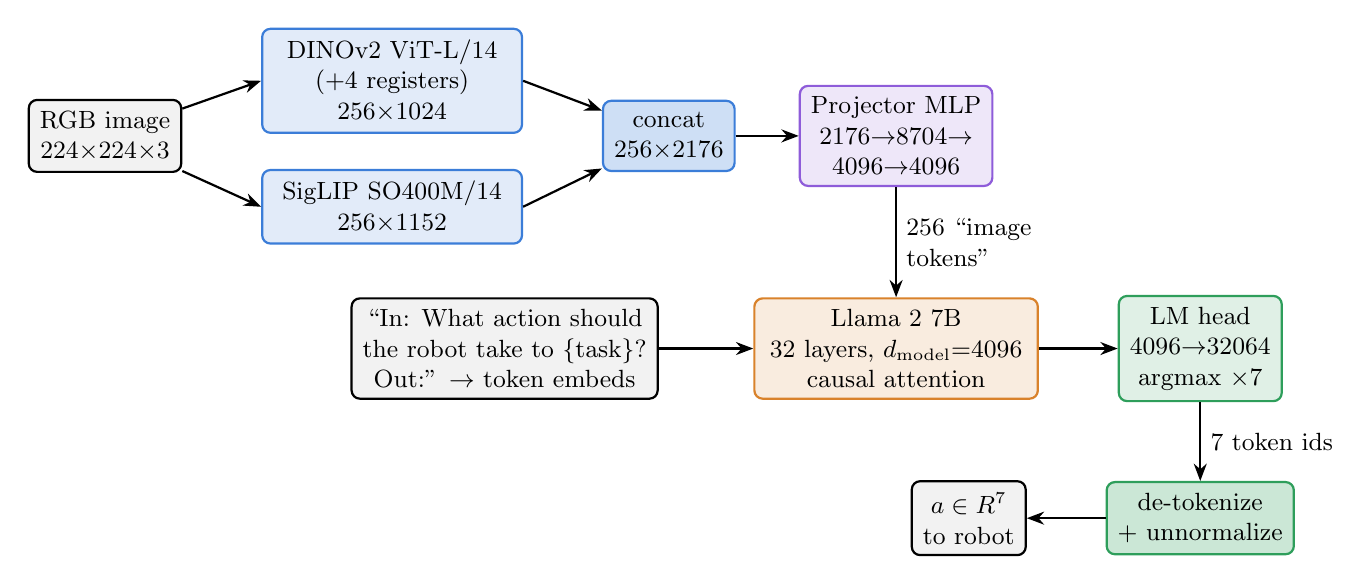
\begin{tikzpicture}[
  font=\small,
  box/.style={draw,rounded corners=3pt,thick,minimum height=8mm,align=center,inner sep=4pt},
  arr/.style={-{Stealth[length=2.2mm]},thick}]
\node[box,fill=black!5] (img) {RGB image\\$224{\times}224{\times}3$};
\node[box,fill=vis!15,draw=vis,right=10mm of img,yshift=7mm,minimum width=33mm] (dino) {DINOv2 ViT-L/14\\(+4 registers)\\$256{\times}1024$};
\node[box,fill=vis!15,draw=vis,right=10mm of img,yshift=-9mm,minimum width=33mm] (sig) {SigLIP SO400M/14\\$256{\times}1152$};
\node[box,fill=vis!25,draw=vis,anchor=west] (cat) at ($(dino.east|-img.east)+(10mm,0)$) {concat\\$256{\times}2176$};
\node[box,fill=proj!15,draw=proj,right=8mm of cat] (mlp) {Projector MLP\\$2176{\to}8704{\to}$\\$4096{\to}4096$};
\node[box,fill=llm!15,draw=llm,below=14mm of mlp,minimum width=36mm] (llama) {Llama 2 7B\\32 layers, $\dm{=}4096$\\causal attention};
\node[box,fill=black!5,left=12mm of llama] (txt) {``In: What action should\\the robot take to \{task\}?\\Out:'' $\to$ token embeds};
\node[box,fill=act!15,draw=act,right=10mm of llama] (head) {LM head\\$4096{\to}32064$\\argmax $\times 7$};
\node[box,fill=act!25,draw=act,below=10mm of head] (det) {de-tokenize\\+ unnormalize};
\node[box,fill=black!5,left=10mm of det] (robot) {$a\in\mathbb{R}^7$\\to robot};
\draw[arr] (img) -- (dino.west);
\draw[arr] (img) -- (sig.west);
\draw[arr] (dino.east) -- (cat);
\draw[arr] (sig.east) -- (cat);
\draw[arr] (cat) -- (mlp);
\draw[arr] (mlp) -- node[right,align=left]{256 ``image\\tokens''} (llama);
\draw[arr] (txt) -- (llama);
\draw[arr] (llama) -- (head);
\draw[arr] (head) -- node[right]{7 token ids} (det);
\draw[arr] (det) -- (robot);
\end{tikzpicture}
\caption{OpenVLA-7B end to end. Colors: blue = vision, purple = projector, orange = language model, green = action read-out. All parameters, including both vision encoders, are trained during VLA training.}
\label{fig:arch}
\end{figure}

\section{Where OpenVLA comes from}

A VLA is easier to explain once you know the ideas it borrows.

\begin{description}[style=nextline,leftmargin=1.2em]
\item[RT-1 (Google, 2022)] A robot transformer trained from scratch on about 130k demonstrations. It introduced \textbf{256-bin discretization of each action dimension}, with actions predicted as classification targets. OpenVLA keeps this scheme.
\item[RT-2 (Google DeepMind, 2023)] Fine-tuned large VLMs (PaLI-X 55B, PaLM-E 12B) to emit action bins \emph{as text tokens}, co-trained with web vision-language data. This is the original ``actions are just language'' VLA. RT-2-X is RT-2 trained on Open X-Embodiment. It was the main closed-source baseline OpenVLA beat.
\item[Open X-Embodiment (2023)] A pooled dataset of 1M+ real-robot trajectories from 22 robot embodiments, in a common RLDS format. OpenVLA trains on a curated 970k-trajectory subset.
\item[Octo (2024)] An open 93M-parameter generalist policy with a \emph{diffusion} action head. Its data-mixture weights were the starting point for OpenVLA's.
\item[Prismatic VLMs (2024)] A controlled study of VLM design choices \cite{karamcheti2024prismatic}. It produced the backbone OpenVLA starts from: fused DINOv2+SigLIP vision, a Llama~2 base model, naive resize, single-stage training.
\item[OpenVLA (June 2024)] Kim, Pertsch, Karamcheti, et al.\ (Stanford, UC Berkeley, TRI, Google DeepMind, Physical Intelligence, MIT). Prismatic-7B + RT-2-style action tokens + OpenX data, fully open (weights, code, data pipeline).
\item[Successors] OpenVLA-OFT (2025) \cite{kim2025oft} replaces the token output with parallel, continuous, chunked actions (Section~\ref{sec:oft}). $\pi_0$ uses a flow-matching ``action expert''. FAST compresses actions with a DCT before tokenizing. These are mostly reactions to the bottlenecks of OpenVLA's one-token-per-dimension design.
\end{description}

%=====================================================================
\part{The Forward Pass, Component by Component}
%=====================================================================

\section{Inputs}

\subsection{Image preprocessing}
\begin{itemize}
  \item \textbf{One image, one camera, one time step.} OpenVLA takes a single third-person RGB frame. It has no wrist camera, no proprioception (joint angles or gripper width), and no history of past frames or actions. The released \texttt{norm\_stats} even store \texttt{proprio} statistics as all zeros.
  \item \textbf{Resize.} The image is resized directly to $224\times224$ (\texttt{image\_resize\_strategy = "resize-naive"}), without cropping or letterboxing. The authors also tried $384\times384$. It gave no measurable improvement and trained about $3\times$ slower.
  \item \textbf{Two normalizations, one tensor.} Each encoder expects different pixel statistics: ImageNet mean/std for DINOv2, mean = std = 0.5 for SigLIP. The processor normalizes the same image twice and stacks the results along the channel axis, so \texttt{pixel\_values} has shape $[B,\,6,\,224,\,224]$. The model splits it back into two 3-channel images.
  \item \textbf{Augmentation.} During training, each image gets a random crop covering 90\% of its area, resized back to 224. At test time you therefore take a \emph{center} 90\% crop (\texttt{-{}-center\_crop True} in the LIBERO scripts). Skipping this measurably lowers success.
\end{itemize}

\subsection{Prompt}
The text input is always the same template, with the task instruction filled in:
\begin{lstlisting}[language={}]
In: What action should the robot take to {instruction}?
Out:
\end{lstlisting}
The Llama SentencePiece tokenizer adds a \texttt{<s>} (BOS, id 1) at the start. At training time the target text \texttt{"Out: <7 action tokens></s>"} tokenizes the space after ``\texttt{Out:}'' as a separate token, id \textbf{29871} (``\texttt{\_}''). At inference, \texttt{predict\_action} therefore appends token 29871 if the prompt doesn't already end with it, so the model sees exactly the prefix it was trained on. The first action token is predicted at the position of token 29871.

\section{Vision encoders: DINOv2 + SigLIP}

\begin{center}
{\small\begin{tabularx}{\linewidth}{@{}lXX@{}}
\toprule
 & DINOv2 & SigLIP \\
\midrule
timm id & \texttt{\footnotesize vit\_large\_patch14\_reg4\_dinov2\allowbreak.lvd142m} & \texttt{\footnotesize vit\_so400m\_patch14\_siglip\_224} \\
Architecture & ViT-L/14, 24 blocks, width 1024 & ViT-SO400M/14, 27 blocks, width 1152 \\
Pretraining & Self-supervised (image-only), LVD-142M & Contrastive image--text (sigmoid loss) \\
What it is good at & Geometry, spatial layout, part structure & Semantics, object categories, language alignment \\
Extra tokens & CLS + 4 \emph{register} tokens (discarded) & none (no CLS) \\
Output used & patch tokens of the 2nd-to-last block & patch tokens of the 2nd-to-last block \\
Output shape & $256\times1024$ & $256\times1152$ \\
\bottomrule
\end{tabularx}}
\end{center}

\paragraph{Patch grid.} With patch size 14 at $224\times224$, each encoder sees a $16\times16$ grid, so \textbf{256 patches}. Each patch covers $14\times14$ pixels. Patch $i$ in DINOv2 and patch $i$ in SigLIP cover the same pixels, so their features can be concatenated per patch: $1024+1152=\mathbf{2176}$ dimensions per patch. The code is literally \texttt{torch.cat([patches, patches\_fused], dim=2)}.

\paragraph{Why the penultimate layer?} Both featurizers call \texttt{get\_intermediate\_layers(n=\{len(blocks)-2\})}. The last block of a pretrained ViT is specialized for its pretraining objective (e.g.\ the contrastive head). The second-to-last block is a more general-purpose representation. This convention comes from LLaVA.

\paragraph{Why two encoders?} Prismatic \cite{karamcheti2024prismatic} found that contrastive encoders (CLIP, SigLIP) beat DINOv2 alone on VLM benchmarks. \emph{Adding} DINOv2 features to SigLIP still gave significant gains, 5--10\% on localization-heavy tasks. For robots, spatial precision matters even more. OpenVLA's ablation trained on Bridge only: dropping DINOv2 (SigLIP alone) cost about 5 points of success (45.6\% $\to$ 40.6\%).

\begin{mental}[: the two encoders]
SigLIP tells the model \emph{what} things are (``a black bowl, a plate''). DINOv2 tells it \emph{where} things are and how they're shaped. Concatenation means every image token carries both kinds of description of one $14\times14$ pixel square.
\end{mental}

\section{The projector}

The fused-backbone projector is a 3-layer MLP applied independently to each patch:
\begin{equation}
z_i = W_3\,\mathrm{GELU}\!\big(W_2\,\mathrm{GELU}(W_1 v_i + b_1) + b_2\big) + b_3,
\qquad v_i\in\mathbb{R}^{2176},\; z_i\in\mathbb{R}^{4096}
\end{equation}
with $W_1: 2176\to 8704$ ($4\times$ expansion), $W_2: 8704\to4096$, $W_3: 4096\to4096$. That is about 71M parameters. The paper calls it a ``2-layer MLP''. The released fused variant has three linear layers, as above. Its only job is to put visual features into the same vector space as Llama's word embeddings, so the language model can treat them like words. It does not mix information between patches: there is no attention and no pooling, and 256 vectors go in and 256 come out.

\section{Assembling the sequence}

The projected patches are spliced in \emph{right after BOS}:
\begin{lstlisting}
# Prismatic defaults to inserting after <BOS> token (1:)
multimodal_embeddings = torch.cat(
    [input_embeddings[:, :1, :], projected_patch_embeddings, input_embeddings[:, 1:, :]], dim=1)
\end{lstlisting}
Patch positions get attention mask \texttt{True} and label \texttt{-100}, so the loss ignores them.

\begin{figure}[h]
\centering
\resizebox{\linewidth}{!}{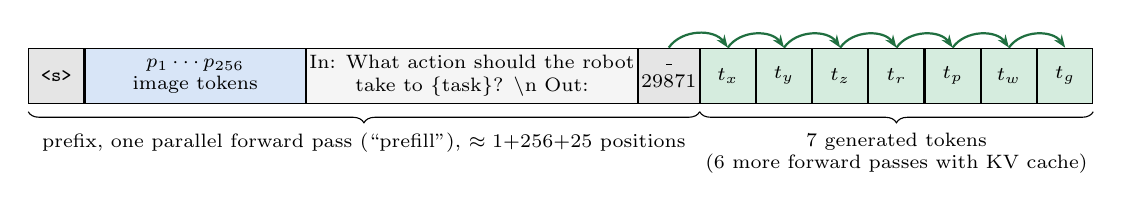
\begin{tikzpicture}[font=\scriptsize,
  tok/.style={draw,minimum height=7mm,minimum width=7mm,inner sep=1pt,align=center},
  arr/.style={-{Stealth[length=1.6mm]},thick,act!70!black}]
\node[tok,fill=black!10] (bos) {\texttt{<s>}};
\node[tok,fill=vis!20,right=0pt of bos,minimum width=28mm] (img) {$p_1 \cdots p_{256}$\\image tokens};
\node[tok,fill=black!4,right=0pt of img,minimum width=42mm] (pr) {In: What action should the robot\\take to \{task\}? \textbackslash n Out:};
\node[tok,fill=black!10,right=0pt of pr] (sp) {\texttt{\_}\\29871};
\node[tok,fill=act!20,right=0pt of sp] (a1) {$t_x$};
\node[tok,fill=act!20,right=0pt of a1] (a2) {$t_y$};
\node[tok,fill=act!20,right=0pt of a2] (a3) {$t_z$};
\node[tok,fill=act!20,right=0pt of a3] (a4) {$t_{r}$};
\node[tok,fill=act!20,right=0pt of a4] (a5) {$t_{p}$};
\node[tok,fill=act!20,right=0pt of a5] (a6) {$t_{w}$};
\node[tok,fill=act!20,right=0pt of a6] (a7) {$t_g$};
\foreach \s/\t in {sp/a1,a1/a2,a2/a3,a3/a4,a4/a5,a5/a6,a6/a7}{
  \draw[arr] (\s.north) to[bend left=55] (\t.north);}
\draw[decorate,decoration={brace,mirror,amplitude=4pt}] ([yshift=-1mm]bos.south west) -- ([yshift=-1mm]sp.south east)
  node[midway,below=4pt,align=center]{prefix, one parallel forward pass (``prefill''), $\approx 1{+}256{+}25$ positions};
\draw[decorate,decoration={brace,mirror,amplitude=4pt}] ([yshift=-1mm]a1.south west) -- ([yshift=-1mm]a7.south east)
  node[midway,below=4pt,align=center]{7 generated tokens\\(6 more forward passes with KV cache)};
\end{tikzpicture}}
\caption{The token sequence. Green arrows: the residual stream at the \emph{tail} of each arrow produces the logits for the token at its \emph{head}. So $t_x$ is read out at the ``\texttt{\_}'' position, $t_y$ at the $t_x$ position, and so on. During training the 7 ground-truth action tokens and the closing \texttt{</s>} are supervised. Everything else is masked out of the loss.}
\label{fig:seq}
\end{figure}

\begin{interp}[: the causal mask covers the image too]
Llama uses a strictly causal mask, and the image comes \emph{before} the text. Two consequences:
\begin{enumerate}
  \item \textbf{Image tokens never see the instruction.} Inside the LLM, the representations at patch positions are computed without the task text. Any instruction-dependent processing of the scene has to happen at text positions or action positions, which can attend back to the patches.
  \item \textbf{Image tokens are causally ordered in raster order.} Patch 17 can attend to patches 1--16 but not 18--256. The vision encoders already mixed information globally, so this matters less than it sounds. Still, patch positions are not symmetric inside Llama.
\end{enumerate}
\end{interp}

\section{The language model: Llama 2 7B}

\begin{center}
\begin{tabularx}{\linewidth}{@{}lX@{}}
\toprule
Layers & 32 decoder blocks \\
Residual width $\dm$ & 4096 \\
Attention & 32 heads $\times$ 128 dims, multi-head (no GQA at 7B), RoPE positions \\
MLP & SwiGLU, hidden width 11008 \\
Normalization & RMSNorm, pre-norm (before attention and before MLP), plus a final RMSNorm \\
Vocabulary & 32000 real tokens, padded to 32064 (multiple of 64); pad id 32000 \\
Embeddings & \emph{untied}: input embedding matrix $W_E$ and output head $W_U$ are separate \\
Parameters & $\approx$6.7B (of OpenVLA's $\approx$7.2B total) \\
\bottomrule
\end{tabularx}
\end{center}

Each block, in residual-stream form ($x_\ell$ is the stream entering layer $\ell$):
\begin{align}
h_\ell &= x_\ell + \mathrm{Attn}_\ell\big(\mathrm{RMSNorm}(x_\ell)\big)\\
x_{\ell+1} &= h_\ell + W^{\ell}_{\text{down}}\Big(\mathrm{SiLU}\big(W^{\ell}_{\text{gate}}\,\tilde h_\ell\big)\odot W^{\ell}_{\text{up}}\,\tilde h_\ell\Big),\qquad \tilde h_\ell=\mathrm{RMSNorm}(h_\ell)
\end{align}
and the output is
\begin{equation}
\text{logits} = W_U\,\mathrm{RMSNorm}_{\text{final}}(x_{32}) \in \mathbb{R}^{32064}.
\end{equation}
\textbf{Base, not chat.} OpenVLA uses \texttt{meta-llama/Llama-2-7b-hf} (the pure base model, \texttt{llama2-7b-pure}). Prismatic found instruction-tuned LMs gave no benefit and hallucinated more.

\begin{mental}[: the residual stream]
Picture each of the $\sim$290 positions as a 4096-dimensional ``notepad''. The notepad at a patch position starts with a description of one image square. The notepad at a text position starts with a word embedding. Each of the 32 layers \emph{adds} to the notepads. Attention copies information between positions, always from earlier to later. The MLP rewrites information within a position. At the end, the notepad at the ``\texttt{\_}'' position is multiplied by $W_U$ to score all 32064 tokens, and the top score among the action tokens is the bin for $\Delta x$.
\end{mental}

%=====================================================================
\part{Actions as Tokens}
%=====================================================================

\section{From a real action to a token}
\label{sec:tok}

\subsection{Action space}
The training data are mostly 7-DoF \emph{end-effector delta} actions: a change in position $(\Delta x,\Delta y,\Delta z)$, a change in orientation $(\Delta\text{roll},\Delta\text{pitch},\Delta\text{yaw})$, and a gripper command. Datasets are only kept if they have single-arm end-effector control and a third-person camera. The units and scale of the action differ by dataset. That is why normalization is done per dataset.

\subsection{Step 1: normalize to $[-1,1]$ per dataset}
For each dataset $D$ and each dimension $j$, compute the 1st and 99th percentiles $q^{D}_{01,j}, q^{D}_{99,j}$ of the training actions. Map that interval to $[-1,1]$ and clip:
\begin{equation}
\bar a_j = \mathrm{clip}\!\left(2\,\frac{a_j - q_{01,j}}{q_{99,j}-q_{01,j}} - 1,\;-1,\;1\right).
\end{equation}
\textbf{Why quantiles instead of min/max?} One outlier action in a dataset would stretch a min/max range and squeeze all normal actions into a few bins. With quantiles the bins cover where the data actually are. Only the most extreme 2\% of values get clipped. In Bridge, for example, $\Delta x$ has min/max $\approx\pm0.41$ but $q_{01}/q_{99}\approx\pm0.028$. A min/max grid would be 15$\times$ coarser.

\textbf{The gripper is not normalized.} It has \texttt{mask = False} in the stats and is already in $[0,1]$ (0 = close, 1 = open in the OpenVLA training convention).

\subsection{Step 2: discretize into bins}
\begin{lstlisting}
bins = np.linspace(-1, 1, 256)                    # 256 bin EDGES
bin_centers = (bins[:-1] + bins[1:]) / 2.0        # 255 centers
idx = np.digitize(np.clip(a, -1, 1), bins)        # integer in 1..256
token_id = tokenizer.vocab_size - idx             # 32000 - idx -> 31744..31999
\end{lstlisting}

\subsection{Step 3: write the bin as a vocabulary token}
Llama's tokenizer has only 100 reserved special tokens, too few for 256 bins. OpenVLA instead \textbf{overwrites the last 256 tokens of the Llama vocabulary} (ids 31744--31999). The paper describes these as the least-used tokens. They are rare sub-word pieces, and their old meaning is destroyed by training. Their input embeddings and their rows of $W_U$ are then learned as action bins.

\begin{figure}[h]
\centering
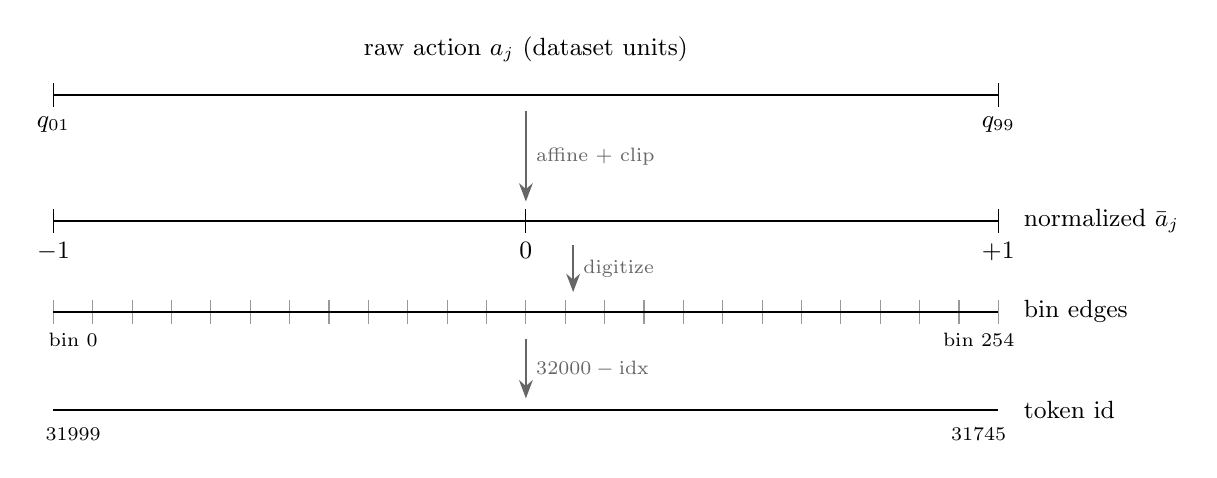
\begin{tikzpicture}[font=\small,x=1cm]
\draw[thick] (0,0) -- (12,0);
\foreach \x/\l in {0/{$q_{01}$},12/{$q_{99}$}} \draw (\x,0.15)--(\x,-0.15) node[below]{\l};
\node[above] at (6,0.3) {raw action $a_j$ (dataset units)};
\draw[thick] (0,-1.6) -- (12,-1.6);
\foreach \x/\l in {0/{$-1$},6/{$0$},12/{$+1$}} \draw (\x,-1.45)--(\x,-1.75) node[below]{\l};
\node[right] at (12.2,-1.6) {normalized $\bar a_j$};
\foreach \i in {0,0.5,...,12} \draw[black!40] (\i,-2.6)--(\i,-2.9);
\draw[thick] (0,-2.75) -- (12,-2.75);
\node[right] at (12.2,-2.75) {bin edges};
\node[below] at (0.25,-2.9) {\scriptsize bin 0};
\node[below] at (11.75,-2.9) {\scriptsize bin 254};
\draw[thick] (0,-4.0) -- (12,-4.0);
\node[below] at (0.25,-4.1) {\scriptsize 31999};
\node[below] at (11.75,-4.1) {\scriptsize 31745};
\node[right] at (12.2,-4.0) {token id};
\draw[-{Stealth},thick,black!60] (6,-0.2) -- (6,-1.35) node[midway,right]{\scriptsize affine + clip};
\draw[-{Stealth},thick,black!60] (6.6,-1.9) -- (6.6,-2.5) node[midway,right]{\scriptsize digitize};
\draw[-{Stealth},thick,black!60] (6,-3.1) -- (6,-3.85) node[midway,right]{\scriptsize $32000-\text{idx}$};
\end{tikzpicture}
\caption{The tokenization chain for one action dimension. Note the \textbf{reversal}: \emph{larger} token ids mean \emph{more negative} actions.}
\end{figure}

\section{From tokens back to an action}

\begin{lstlisting}
generated_ids = self.generate(input_ids, max_new_tokens=7, do_sample=False)
ids  = generated_ids[0, -7:]
idx  = np.clip(32000 - ids - 1, 0, 254)          # bin index into 255 centers
norm = bin_centers[idx]                          # in [-1, 1]
a    = np.where(mask, 0.5*(norm+1)*(q99-q01) + q01, norm)   # unnormalize
\end{lstlisting}
\begin{itemize}
  \item \textbf{Decoding is greedy} (\texttt{do\_sample=False}): argmax at each of 7 steps, each conditioned on the previous action tokens.
  \item \textbf{The argmax runs over all 32064 logits}, not only the 256 action rows. A trained model essentially always picks an action token. If it didn't, the clip would silently turn the stray token into an edge bin.
  \item \textbf{Which statistics?} \texttt{unnorm\_key} picks the dataset whose $q_{01}/q_{99}$ are used, e.g.\ \texttt{"bridge\_orig"} for the base model or \texttt{"libero\_spatial"} for the LIBERO checkpoint. The \emph{same} token means a different physical motion under different keys.
  \item \textbf{Resolution.} One bin is $2/255$ of the normalized range, or $(q_{99}-q_{01})/255$ in raw units. In your run 2 data that is about 0.006--0.007 for translation.
\end{itemize}

\begin{pitfall}[: ``256 bins'']
The paper says 256 bins, and 256 token ids are reserved. The code builds 256 bin \emph{edges}, so there are only 255 \emph{centers}. On decode, ids 31744 and 31745 both map to the last center ($+0.996$). In practice the model has 255 distinct output values per dimension, and the lowest token id is effectively a duplicate. When your logit lens takes a softmax over ``256 action bins'', keep in mind that two of those rows decode to the same value.
\end{pitfall}

\begin{pitfall}[: the 7 dimensions are independent outputs]
They are \emph{not} independent. Generation is autoregressive in the fixed order $x,y,z,\text{roll},\text{pitch},\text{yaw},\text{gripper}$. The gripper token is predicted with the first six already in context. During training this was teacher-forced on the \emph{ground-truth} previous dimensions. At test time the model conditions on its \emph{own} previous predictions.
\end{pitfall}

%=====================================================================
\part{Training}
%=====================================================================

\section{Data: Open X-Embodiment, curated}

\begin{itemize}
  \item \textbf{Source.} Open X-Embodiment (OpenX): 70+ datasets, 2M+ trajectories when the paper was written.
  \item \textbf{Curation.} Keep only manipulation datasets with $\ge 1$ third-person camera and single-arm end-effector control. Result: \textbf{970k trajectories} across about 25 datasets (the 25 \texttt{norm\_stats} keys in the released config).
  \item \textbf{Mixture weights.} Start from Octo's weights, which down-weight low-diversity datasets and up-weight diverse ones. The largest shares are Bridge 13.3\%, Fractal (RT-1) 12.7\%, and Kuka 12.7\%. DROID was added at 10\% but removed for the last third of training because its action-token accuracy stayed low.
  \item \textbf{Cleaning.} All-zero (no-op) actions in Bridge were filtered out.
  \item \textbf{No web data.} Unlike RT-2, OpenVLA does \emph{not} co-train with internet vision-language data during robot training. Its ``world knowledge'' comes only from the pretrained Prismatic weights it starts from.
\end{itemize}

\section{Objective}

Standard next-token cross-entropy, computed \textbf{only on the action tokens} (and the closing \texttt{</s>}):
\begin{equation}
\mathcal{L} = -\sum_{j=1}^{7}\log p_\theta\big(t_j \mid \text{image},\;\text{prompt},\;t_{<j}\big).
\end{equation}
Note what this loss does \emph{not} know: bin 128 and bin 129 are as ``different'' as bin 0 and bin 255. Getting close earns nothing. Any notion that neighboring bins are similar has to be learned from the data. This is one reason successors switched to regression (Section~\ref{sec:oft}).

The training metric reported in the paper is \textbf{action-token accuracy}: the fraction of action tokens whose argmax equals the ground-truth bin, under teacher forcing.

\section{Recipe and compute}

\begin{center}
\begin{tabular}{@{}ll@{}}
\toprule
Initialization & Prismatic-7B (DINOv2+SigLIP, Llama 2 7B), already a VLM \\
Trainable & \textbf{everything}, including both vision encoders \\
Hardware / time & 64 A100 GPUs $\times$ 14 days $\approx$ 21{,}500 A100-hours \\
Batch size & 2048 \\
Learning rate & $2\times10^{-5}$, constant, no warmup (warmup did not help) \\
Epochs & 27 passes over the mix, until training action-token accuracy $>95\%$ \\
Stack & PyTorch, FSDP, FlashAttention, AMP (bf16) \\
\bottomrule
\end{tabular}
\end{center}

\begin{pitfall}[: ``freeze the vision encoder, like VLMs do'']
Prismatic found that fine-tuning the vision encoder \emph{hurt} VLM benchmarks. OpenVLA found the opposite for control: fine-tuning it was crucial. Averaged across their evaluations, fine-tuning reached about 80\% success versus about 47\% with a frozen encoder. The likely reason is that internet-pretrained features are not precise enough about small spatial details (exact gripper--object offsets) for control. 27 epochs is also far more than the usual 1--2 for VLMs. Robot policies need near-exact action-token accuracy.
\end{pitfall}

\section{Design choices the authors tested}

\begin{center}
\begin{tabularx}{\linewidth}{@{}lX@{}}
\toprule
Choice & Finding \\
\midrule
VLM backbone & LLaVA beat IDEFICS-1 by about 35\% absolute on language-grounding tasks. Prismatic beat LLaVA by about 10\%, which the authors credit to the fused SigLIP+DINOv2 encoder. \\
OpenX vs.\ Bridge-only data & Training only on Bridge cost about 30 points on Bridge tasks (76.3\% $\to$ 45.6\%). Cross-embodiment data helps even on the in-domain robot. \\
DINOv2 & Removing it (SigLIP only, Bridge-only training) cost about 5 more points (45.6\% $\to$ 40.6\%). \\
Resolution & 384 px vs.\ 224 px: no gain, about $3\times$ the training compute. \\
Frozen vision & Large drop (above). \\
Epochs & Many more than for VLMs. Success kept improving until token accuracy was above 95\%. \\
\bottomrule
\end{tabularx}
\end{center}

%=====================================================================
\part{Adaptation, Deployment, and Results}
%=====================================================================

\section{Fine-tuning to a new robot or task}

The authors compared fine-tuning strategies on Franka tasks (batch 16):
\begin{center}
\begin{tabular}{@{}lrrr@{}}
\toprule
Strategy & Success & Trainable params & VRAM \\
\midrule
Full fine-tuning & $69.7\pm7.2\%$ & 7{,}188.1M & 163.3 GB \\
Last layer only & $30.3\pm6.1\%$ & 465.1M & 51.4 GB \\
Frozen vision & $47.0\pm6.9\%$ & 6{,}760.4M & 156.2 GB \\
Sandwich (vision + embed + last layer) & $62.1\pm7.9\%$ & 914.2M & 64.0 GB \\
\textbf{LoRA, $r=32$} & $\mathbf{68.2\pm7.5\%}$ & \textbf{97.6M (1.4\%)} & 59.7 GB \\
LoRA, $r=64$ & $68.2\pm7.8\%$ & 195.2M & 60.5 GB \\
\bottomrule
\end{tabular}
\end{center}
LoRA ($r=32$, applied to all linear layers) matches full fine-tuning at 1.4\% of the trainable parameters. It runs in 10--15 hours on one A100, about $8\times$ less compute. All released LIBERO checkpoints were trained this way.

\subsection{The LIBERO recipe (what your checkpoints are)}
\begin{enumerate}
  \item \textbf{Re-render demos at $256\times256$}, up from LIBERO's native $128\times128$.
  \item \textbf{Rotate images 180°}, at train and test time, because LIBERO's renderer returns them upside down.
  \item \textbf{Filter no-op actions}: near-zero translation and rotation with no gripper change. The authors call this crucial. Without it the policy learns to stand still and freezes during evaluation.
  \item \textbf{Drop failed demos} found by replaying them: 68/500 for Spatial, 46 for Object, 72 for Goal, 121 for Long.
  \item \textbf{Third-person camera only.} No wrist camera and no proprioception, for every method compared.
  \item One LoRA-$r{=}32$ checkpoint per suite, e.g.\ \texttt{openvla/openvla-7b-finetuned-libero-spatial}, with its own \texttt{unnorm\_key} (\texttt{libero\_spatial}).
  \item \textbf{Evaluation-time conventions}: center crop (90\% area), then convert the gripper. OpenVLA outputs $[0,1]$. LIBERO expects $-1$ = open and $+1$ = close, so the value is rescaled to $[-1,1]$, binarized, and its sign flipped.
\end{enumerate}

\section{Inference}

\begin{itemize}
  \item \textbf{Cost per control step:} one prefill pass over about 280 positions, then 6 more single-token passes with the KV cache. That is 7 sequential LM-head read-outs per action.
  \item \textbf{Speed and memory:} about 15 GB in bf16, about 6 Hz on an RTX 4090 without compilation or speculative decoding.
  \item \textbf{Quantization} (8 Bridge tasks):
\begin{center}
\begin{tabular}{@{}lrr@{}}
\toprule
Precision & Success & VRAM \\
\midrule
bf16 & $71.3\pm4.8\%$ & 16.8 GB \\
int8 & $58.1\pm5.1\%$ & 10.2 GB \\
int4 & $71.9\pm4.7\%$ & 7.0 GB \\
\bottomrule
\end{tabular}
\end{center}
int8 looks worse only because its kernels were slow (1.2 Hz on an A5000), and the real robot kept moving while the model computed. With blocking control, where the robot waits for each action, the three precisions perform the same (70.0 / 74.4 / 68.8\%).
\end{itemize}

\section{Headline results}

\begin{itemize}
  \item \textbf{Zero-shot generalist control} (BridgeData V2 WidowX, 17 tasks; Google Robot, 12 tasks): OpenVLA beats RT-2-X (55B) by \textbf{16.5\% absolute} averaged over 29 tasks, with $7\times$ fewer parameters. It outperforms RT-2-X in every category except \emph{semantic} generalization, where RT-2-X's web co-training helps.
  \item \textbf{Fine-tuning to new setups} (Franka): about 20\% better than Diffusion Policy trained from scratch, and the only method with $\ge50\%$ success on every task. Diffusion Policy is still smoother on narrow, dexterous single-instruction tasks.
  \item \textbf{LIBERO} (500 trials per suite, 3 seeds):
\begin{center}
\begin{tabular}{@{}lccccc@{}}
\toprule
Method & Spatial & Object & Goal & Long & Avg \\
\midrule
Diffusion Policy (scratch) & 78.3 & \textbf{92.5} & 68.3 & 50.5 & 72.4 \\
Octo (fine-tuned) & 78.9 & 85.7 & \textbf{84.6} & 51.1 & 75.1 \\
OpenVLA (LoRA) & \textbf{84.7} & 88.4 & 79.2 & \textbf{53.7} & \textbf{76.5} \\
\midrule
OpenVLA-OFT & \multicolumn{4}{c}{(reported average)} & 97.1 \\
\bottomrule
\end{tabular}
\end{center}
Your run 2 (42/50 = 84.0\% on Spatial) is consistent with the reported 84.7\%.
\end{itemize}

\section{Limitations and what came next}
\label{sec:oft}

\paragraph{Limitations stated by the authors.} Single image only: no history, no proprioception, no wrist camera. Throughput is too low for high-frequency control such as ALOHA at 50 Hz. Reliability is usually below 90\%. Open questions remain about base-VLM size and whether web co-training helps.

\paragraph{Structural bottlenecks of the token design.}
(1)~\emph{Sequential decoding}: 7 forward passes per action. (2)~\emph{Discretization}: 255 values per dimension, and a loss that ignores how close a wrong bin is. (3)~\emph{One step at a time}: no action chunking, so motion can be jerky and small errors compound.

\paragraph{OpenVLA-OFT (Kim, Finn, Liang, 2025)} \cite{kim2025oft} keeps the same backbone and changes the action interface:
\begin{itemize}
  \item \textbf{Parallel decoding}: feed empty action placeholder embeddings and use \emph{bidirectional} attention over them, so all action dimensions come out in one forward pass.
  \item \textbf{Action chunking}: predict $K$ future actions at once ($K=8$ on LIBERO).
  \item \textbf{Continuous actions}: an MLP head on the final hidden states replaces the LM head and bins.
  \item \textbf{L1 regression loss} in place of cross-entropy. It matches diffusion heads on success while training and running faster.
  \item Optional extra inputs (wrist camera, proprioception). The OFT+ variant adds FiLM language conditioning for bimanual ALOHA.
\end{itemize}
Result: LIBERO average 76.5\% $\to$ 97.1\%, and about $26\times$ action-generation throughput.

%=====================================================================
\part{Mental Model for Interpretability}
%=====================================================================

\section{Tensor-shape cheat sheet (batch 1)}

\begin{center}
\begin{tabular}{@{}lll@{}}
\toprule
Stage & Shape & Notes \\
\midrule
Env frame (LIBERO) & $256\times256\times3$ & rotate 180°, center crop 90\%, resize \\
\texttt{pixel\_values} & $[1,6,224,224]$ & DINOv2-normed $\Vert$ SigLIP-normed \\
DINOv2 patches & $[1,256,1024]$ & block 22 of 24 (0-indexed); CLS + registers dropped \\
SigLIP patches & $[1,256,1152]$ & block 25 of 27 (0-indexed) \\
Fused features & $[1,256,2176]$ & concat on feature dim \\
Projected & $[1,256,4096]$ & 3-layer GELU MLP \\
LLM input & $[1,\,1{+}256{+}T,\,4096]$ & $T\approx$ 20--35 prompt tokens incl.\ 29871 \\
Residual stream $x_\ell$ & same & $\ell=0$ (embeddings) $\ldots$ 32 \\
Logits & $[1,L,32064]$ & action rows: ids 31744--31999 \\
Output & $\mathbb{R}^7$ & after de-tokenize + unnormalize + gripper convention \\
\bottomrule
\end{tabular}
\end{center}

\section{Where to look, and what each probe means}

\begin{interp}[: reading action predictions from inside]
\begin{itemize}
  \item \textbf{Which position?} The prediction for action dimension $j$ (1-indexed) is read from position $P_{\text{end}}+j-1$, where $P_{\text{end}}$ is the ``\texttt{\_}'' (29871) position. Dimension $x$ is read at a \emph{text} position. Dimensions $y$ through gripper are read at \emph{action-token} positions, whose input embeddings are learned bin embeddings.
  \item \textbf{Logit lens on actions.} $\;\text{logit-lens}_\ell = W_U[\,31744{:}32000\,]\cdot\mathrm{RMSNorm}_{\text{final}}(x_\ell)$. You need the final RMSNorm, because the stream's scale grows with depth. Restricting to the 256 action rows (your run 2 setup) answers ``which bin would the model pick now?'' and ignores whether a text token would have won.
  \item \textbf{Untied embeddings.} When you analyze action tokens as \emph{inputs} (e.g.\ the $x$-token feeding the $y$ prediction), the relevant vector is a row of $W_E$, not $W_U$. These are different learned vectors.
  \item \textbf{Bin geometry.} Cross-entropy does not force neighboring bins to have similar $W_U$ rows. Whether they end up ordered (e.g.\ lying near a 1-D curve) is an empirical question, and a cheap first analysis.
  \item \textbf{Markov policy.} With no history in the input, any temporal consistency you see across steps (e.g.\ a gripper that stays closed) has to be recomputed from the current image each step.
  \item \textbf{Image tokens are instruction-blind} (causal mask). Probing patch positions for task identity should fail by construction. Probing text or action positions for scene properties should succeed.
  \item \textbf{FFN value vectors.} Häon et al.\ (CoRL 2025) \cite{haon2025steering} project rows of $W_{\text{down}}$ through the unembedding into token space. They find sparse, semantically meaningful directions in OpenVLA and $\pi_0$ (e.g.\ speed, direction) and steer behavior by injecting them at inference time. This is the natural causal follow-up to logit-lens observations.
\end{itemize}
\end{interp}

\section{The two-minute spoken explanation}

\begin{quote}
``OpenVLA is a vision-language model repurposed as a robot policy. It starts from Prismatic, a LLaVA-style VLM. Two vision transformers, DINOv2 for spatial structure and SigLIP for semantics, each turn a $224\times224$ camera image into a $16\times16$ grid of patch features. Those are concatenated and passed through a small MLP into Llama~2's embedding space. That gives 256 visual tokens, placed right after the start token and before a fixed prompt: `What action should the robot take to \textit{[instruction]}?' Llama~2 7B processes the sequence causally, and the language-model head generates seven tokens. Each one is a bin index for one action dimension: three position deltas, three rotation deltas, and the gripper. To fit them in the vocabulary, the authors overwrote the 256 least-used Llama tokens. Each action dimension is normalized per dataset with its 1st and 99th percentiles and cut into uniform bins, and at test time that mapping is inverted. The whole 7B model, vision encoders included, was trained with plain cross-entropy on 970k Open X-Embodiment trajectories for 27 epochs on 64 A100s. It beats the 55B RT-2-X by 16.5 points. It adapts to new robots with LoRA at 1.4\% of the parameters and gets about 77\% on LIBERO. Its main limits come from the token interface: seven sequential decoding steps, discretized actions, no history, and no chunking. OpenVLA-OFT fixes these with parallel decoding of continuous action chunks trained with an L1 loss.''
\end{quote}

\section{Self-test questions}

\begin{enumerate}
  \item Why does OpenVLA concatenate DINOv2 and SigLIP features instead of using one encoder? What did the ablation cost when DINOv2 was removed?
  \item Where exactly are image tokens inserted in the sequence? Can a patch token attend to the instruction?
  \item Write the formula mapping a raw action value to a token id. Why use $q_{01}/q_{99}$ instead of min/max?
  \item How many distinct values can one action dimension take at output? Why is the answer not 256?
  \item At which sequence position is the gripper token predicted? What has the model already written by then?
  \item What does \texttt{unnorm\_key} do, and why does it matter?
  \item VLMs often freeze the vision encoder. Why did OpenVLA fine-tune it, and what was the effect?
  \item Why does cross-entropy over bins lose information compared with L1 regression? How did OpenVLA-OFT change the output head?
  \item Why did int8 quantization look worse than int4 on the real robot, and how was that confirmed?
  \item Name three steps in the LIBERO fine-tuning recipe that are not about the model at all (data or evaluation conventions).
\end{enumerate}

\section{Sources}
\label{sec:sources}

\begin{thebibliography}{9}
\bibitem{kim2024openvla} M.~J. Kim, K.~Pertsch, S.~Karamcheti, et al.
\emph{OpenVLA: An Open-Source Vision-Language-Action Model.} CoRL 2024. \url{https://arxiv.org/abs/2406.09246}

\bibitem{karamcheti2024prismatic} S.~Karamcheti, S.~Nair, A.~Balakrishna, P.~Liang, T.~Kollar, D.~Sadigh.
\emph{Prismatic VLMs: Investigating the Design Space of Visually-Conditioned Language Models.} ICML 2024. \url{https://arxiv.org/abs/2402.07865}

\bibitem{kim2025oft} M.~J. Kim, C.~Finn, P.~Liang.
\emph{Fine-Tuning Vision-Language-Action Models: Optimizing Speed and Success} (OpenVLA-OFT). RSS 2025. \url{https://arxiv.org/abs/2502.19645}

\bibitem{haon2025steering} B.~Häon, K.~Stocking, I.~Chuang, C.~Tomlin.
\emph{Mechanistic Interpretability for Steering Vision-Language-Action Models.} CoRL 2025. \url{https://arxiv.org/abs/2509.00328}

\bibitem{hfcode} OpenVLA release code and config: \url{https://huggingface.co/openvla/openvla-7b} (\texttt{modeling\_prismatic.py}, \texttt{config.json}); \url{https://github.com/openvla/openvla} (\texttt{prismatic/vla/action\_tokenizer.py}, LIBERO eval scripts).
\end{thebibliography}

\noindent\small Background on RT-1, RT-2, Open X-Embodiment, Octo, $\pi_0$ and FAST is summarized from general knowledge of those papers, not re-read for this guide. Llama~2 internals (layer count, widths, RMSNorm, SwiGLU, untied embeddings) come from the public Llama~2 7B configuration.

\end{document}
